\newpage
\chapter{Electrical Infrastructure}

\section{Introduction}
\vspace{-2mm}
In this chapter, the proposed electrical and electronic infrastructure model will be thoroughly examined---purely from a hardware/electronics perspective; along with the development objectives in mind to achieve the desired performance.

\section{Development Objectives}
The electrical infrastructure acts as the "brawn" for the robot, whether as energy source or in outside-world interactions. Providing the suitable power source is essential to ensure both the functionalities of the processing unit and the existing auxiliary units. Therefore, the main objectives for the infrastructure can be summarized as follows:
\begin{itemize}
    \item Providing a stable power source to the whole system.
    \item Providing the means for data acquisition outside the robot.
    \item Providing the means for physical manipulation.
\end{itemize}
Based on the decided objectives, the infrastructure should capable of:
\begin{itemize}
    \item Reliable Power Management and Delivery. 
\end{itemize}
% *six hours later*
% The

%% I am really struggling.
\vspace{-1mm}
\section{Design Approach}\label{sect:d_approach}
Connecting the battery pack directly to the system is not a plausible option, due to the need for different voltage levels for operation, mainly 12 and 5 volts. Moreover, monitoring the status of the battery pack and providing a controlled environment for its operation ensure a safer operation.
\newline This approach can be represented as in diagram \ref{fig:hw-power-blk1}, where the selected battery pack is connected to a BMS, which is connected to the processing unit for data acquisition. After being processed, the power goes to a distribution system to provide the suitable voltage levels to the system. 

\newpage

\begin{figure}[h!]
    \centering
    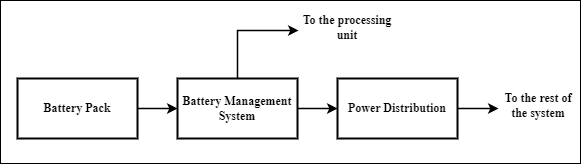
\includegraphics[scale=0.5]{./Figures/HW/powerDiagram-drawio.png}
    \caption{The Block Diagram for Power Management.}
    \label{fig:hw-power-blk1}
\end{figure}


% I will adjust this one if necessary so that
%no other figure suffers the same fate

For the \textbf{BMS}, a smart architecture is proposed . It should use a hardware-based protection  system for over-voltage, under-voltage, over-current and short-circuit for faster response. 
\newline A controller is present for measuring voltages, current, and temperature of the pack, and send it to the processing unit to be sent to the end-user. \cite{bms_david}\textbf{Power distribution} should provide 12V for motion, as well as 5V with high current capabilities for to power the processing unit and other subsystems.

% Imagine there is a block diagram for the BMS

\section{Proposed Design }
% Based on the used components and modules, as well as the need for a compact system, a battery-pack of 3 18650 cells in series is used to produce up to 12.6V at full charge. 
\subsection{Battery Pack}\label{subsection:battery}
% Starting from the top, the battery pack was built initially to satisfy the need of the most voltage-demanding component: the motors, which are rated for 12 V. Another important aspect regarding the used cell in the pack is its energy density, where it is desired to choose a high energy density battery for a more compact design. For these reasons, the pack is built using Lithium-Ion (Li-ion) batteries, specifically the 18650 package. \cite{cellComp}

Starting from the top, it is desired to build the battery pack with high gravimetric and volumetric energy densities for a compact pack running for a long time, so it was built using the 18650 Lithium-Ion (Li-ion) cells. \cite{cellComp}

% For satisfying the need of the most voltage-demanding component: the motors; which are rated for 12V, the pack is built using 3 cells in series, acheiving ov

Other important aspects of the pack are its nominal voltage and capacity, where they depend on the highest voltage-demand of the circuit and desired run-time. At full-load, the robot requires up to \textbf{51.25 W} of power, and for a runtime of about \textbf{1 hr}, according the relation \ref{equ:runtime}:
\begin{equation}
    Runtime = \frac{Energy\ Capacity\ at\ full\ charge[Wh]}{Consumed\ Power\ at\ Full-Load[W]}
    \label{equ:runtime}
\end{equation}
A pack of energy capacity \textbf{51.25 Wh} is required. Since the energy capacity is a function of the voltage of the pack as in relation \ref{equ:energy-capacity}, we can determine the overall charge capacity, measured in \textbf{Ah}, where:
\begin{itemize}
    \item $n_s$: number of cells or modules in series.
    \item $n_p$: number of cells or modules in parallel.
    \item $C_{cell}$: Charge capacity of one cell \textbf{[Ah]}
    \item $V_{cell}$: Voltage of one cell \textbf{[V]}
\end{itemize}
\newpage
\begin{equation}
    Energy\ Capacity[Wh] = n_s * n_p * C_{cell} * V_{cell}
    \label{equ:energy-capacity}
\end{equation} % I have returned!
\textbf{$V_{cell}$} of each 18650 Li-ion battery can be up to \textbf{4.2 V} at full-charge, and to satisfy the need of the most voltage demanding component: the motors; which are rated for \textbf{12 V}, the pack is built using \textbf{3} cells in series, to obtain \textbf{12.6 V} at full-charge. Therefore, the charge capacity of each cell is about \textbf{4.067 Ah}. 

\begin{figure}[h!]
    \centering
    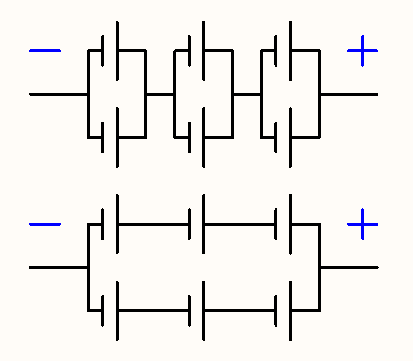
\includegraphics[scale=0.5]{./Figures/HW/cell-configs.png}
    \caption{Hybrid cell configurations in a pack.}
    \label{fig:hw-cell-config}
\end{figure}


To use a cell with a commercially-available capacity, parallel connections can be used. As shown in figure \ref{fig:hw-cell-config}, cells are either connected in parallel; forming modules to be connected in series (as in the top figure), or modules of series-connected cells are connected in parallel (as in the bottom figure). These configurations hold the naming convention: \{ $n_s$ ($n_p$) modules and $n_p$($n_s$) cells\}. In this case, these configurations are called \textbf{3S2P} and \textbf{2P3S} respectively. For the sake of simplicity in monitoring, the former configuration is used.\newline From the local market, the best choice for Li-ion cells was the \textbf{BESTON} Li-ion cells with nominal capacity of \textbf{2600 mAh}. Connecting 2 cells in parallel formed a module of capacity \textbf{5200 mAh}, for a total energy capacity of \textbf{65.52 Wh} for about 1 hour and 15 minutes of runtime, which was enough for the prototype.
% welcome bacc
% btw I will make a few adjustments to chapter sectioning. do not panik. it will be more convenient that way
\subsection{Battery Management System}
\label{sec:bat-man}


 % From the objectives defined in section , a simple  for the 
Previously in section \ref{sect:d_approach}, the main objectives for the BMS are defined, thus each one can be achieved using abstracted subsystems, as shown in figure \ref{fig:hw-power-blk2}. Monitoring the pack status provides the user with information regarding its health, charge and discharge rate, and any possible problem with the pack.
\newpage
\begin{figure}[h!]
	\centering
	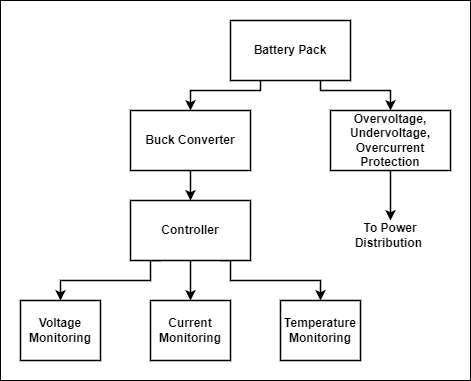
\includegraphics[scale=0.5]{./Figures/HW/BMS-drawing.png}
	\caption{The block diagram of the suggested BMS}
	\label{fig:hw-power-blk2}
\end{figure}

 For the choice of the controller, It was decided to use the ESP32. % I would need some assistance here

% my final message
    %save the world

\textbf{Voltage measurement} depends on the basic idea of \textbf{voltage dividers} as shown in figure \ref{fig:hw-volt-mes} .Each module of the pack (refer to the upper schematic in figure \ref{fig:hw-cell-config}) feeds two resistors in series, and the middle voltage is measured by the controller. Voltages of 4.2, 8.4, 12.6 volts at full-charge are converted to voltages suitable for the ADC of the controller. Based on calculations in the \textbf{Appendix B}, the minimum values of $\frac{R_1}{R_2}$, $\frac{R_3}{R_4}$, and $\frac{R_5}{R_6}$ are $\frac{3}{11}$,$\frac{17}{11}$, and $\frac{31}{11}$ respectively.

\begin{figure}[h!]
    \centering
    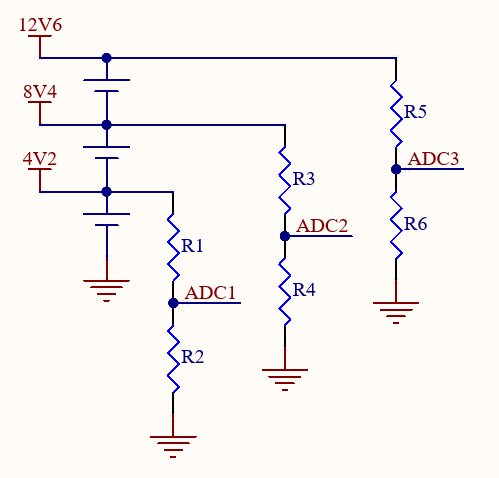
\includegraphics[scale=0.65]{./Figures/HW/Voltage-Measurement.png}
    \caption{Voltage Measurement Using Voltage Divider.}
    \label{fig:hw-volt-mes}
\end{figure}

 
\newpage
% %A figure demonstrating the voltage dividers is to be added




\textbf{Current measurement} had two approaches: using a voltage-drop method or a hall-effect sensor. For the sake of simplicity and cost, the voltage-drop approach is chosen, as shown in figure \ref{fig:hw-current-mes}. Its concept depends on measuring the voltage drop across \textbf{$R_{Shunt}$}, and calculating current knowing the value of the resistor. Some issues arise from this approach are:
\begin{itemize}
    \item The voltage across \textbf{$R_{Shunt}$} may exceed the maximum voltage the ADC can handle.
    \item If \textbf{$R_{Shunt}$} is too high, the power loss across \textbf{$R_{Shunt}$} can be a considerable loss, and even exceed its power rating.
    \item If \textbf{$R_{Shunt}$} is too low, the measured voltage range can be quite low, and inaccuracies might occur.
\end{itemize}



\begin{figure}[h!]
	\centering
	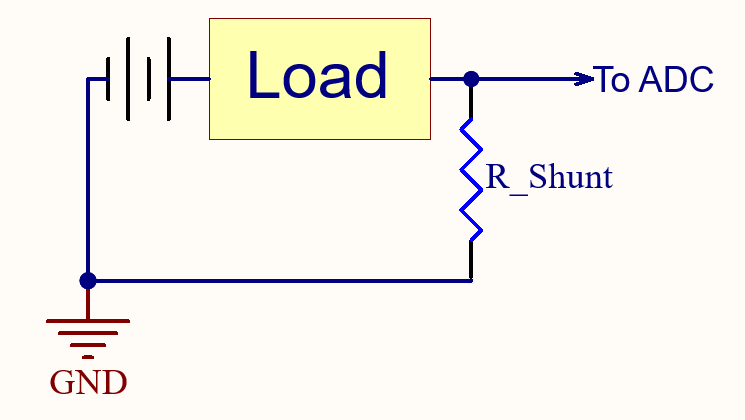
\includegraphics[scale=0.4]{./Figures/HW/Current-Measurement.png}
	\caption{The voltage drop method of current measurement.}
	\label{fig:hw-current-mes}
\end{figure}


\textbf{Alternate solution:} Using a low resistance shunt of high power rating, and the voltage across it is fed to a rail-to-rail Op-Amp with a non-inverting amplifier configuration, as shown in figure \ref{fig:hw-current-mes-2}. This will ensure a low voltage drop across \textbf{$R_{Shunt}$} and a wide range of measured voltage for better accuracy. 

\begin{figure}[h!]
    \centering
    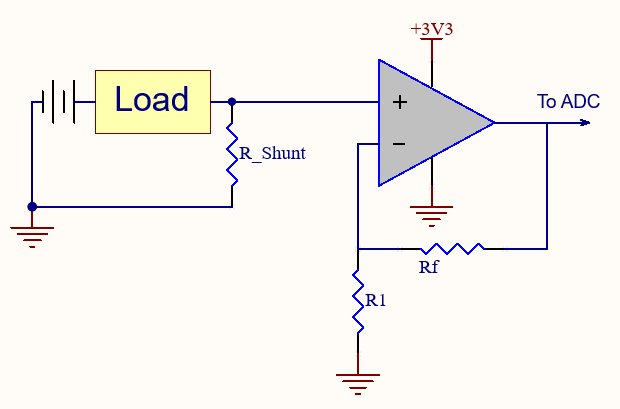
\includegraphics[scale=0.5]{./Figures/HW/Improved-Current-Measurement.png}
    \caption{Improved Current Measurement Using Voltage Drop Method.}
    \label{fig:hw-current-mes-2}
\end{figure}

Applying that design concept, the component values were chosen accordingly. \textbf{$R_{Shunt} = 0.05 \Omega$} for a voltage drop up to \textbf{0.2 V} and power loss of \textbf{0.8 W} at a current draw of \textbf{4 A}. 

\newpage

The values of Op-Amp resistors \textbf{$R_1$} and \textbf{$R_f$} are \textbf{$15 k\Omega$} and \textbf{$150 k\Omega$} for a voltage gain of \textbf{11} and a measured voltage of \textbf{2.2 V} which is fine for the ADC and provides a room for measuring higher current should it exist. The Op-Amp of choice is \textbf{MCP6002}: a rail-to-rail Op-Amp with $V_{CC}$ = \textbf{3.3 V} should provide output voltages up to almost its $V_{CC}$. 

\begin{figure}[h!]
    \centering
    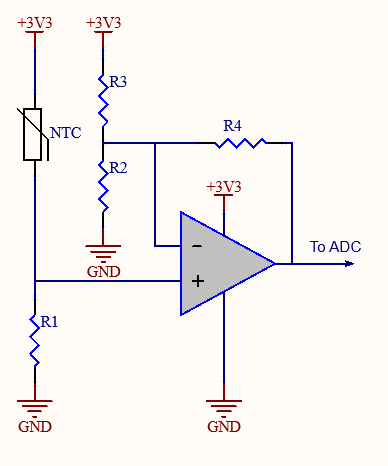
\includegraphics[scale=0.65]{./Figures/HW/Temperature-Measurement.png}
    \caption{Temperature Measurement Using Op-Amp.\cite{op_amp_temperature}}
    \label{fig:hw-temp-mes}
\end{figure}

\textbf{Temperature measurement} 
can be done using a voltage divider circuit with one of the resistors being an NTC resistor. One issue is the narrow range of the output voltage of the voltage divider. One way to remedy this is using an Op-Amp to widen its range, utilizing the full ADC resolution. \cite{op_amp_temperature} 

Using the calculations provided in document \cite{op_amp_temperature}, the values of resistors are calculated to be: \textbf{$R_1 = 78 k\Omega$}, \textbf{$R_2 = 47 k\Omega$}, \textbf{$R_3 = 56 k\Omega$}, and \textbf{$R_4 = 68 k\Omega$}. 

For achieving the protection features, a commercial 3S BMS module is used, capable of overvoltage, undervoltage, and over-current protection. However, one missing crucial feature of the BMS module is cell-balancing, which allows the cells of the pack itself to charge equally should there exist a difference in their capacity. This circuit uses information from voltage sensing subsystem, and open a path for each module to a dummy load if there exist an imbalance of charge.
\newline The cell-balancing circuit is as shown in figure \ref{fig:hw-balance-circuit}. All shown components are used in the actual circuit, except for the MOSFET, which is replaced by SI2302. The circuit simulates the pins of the ESP32, each pin controls an optocoupler to activate a MOSFET, which allows each module (the individual cell in the simulation) to discharge through a resistor The shown results of the simulation in figure \ref{fig:hw-balance-results}.

\newpage 

\begin{figure}[h!]
    \centering
    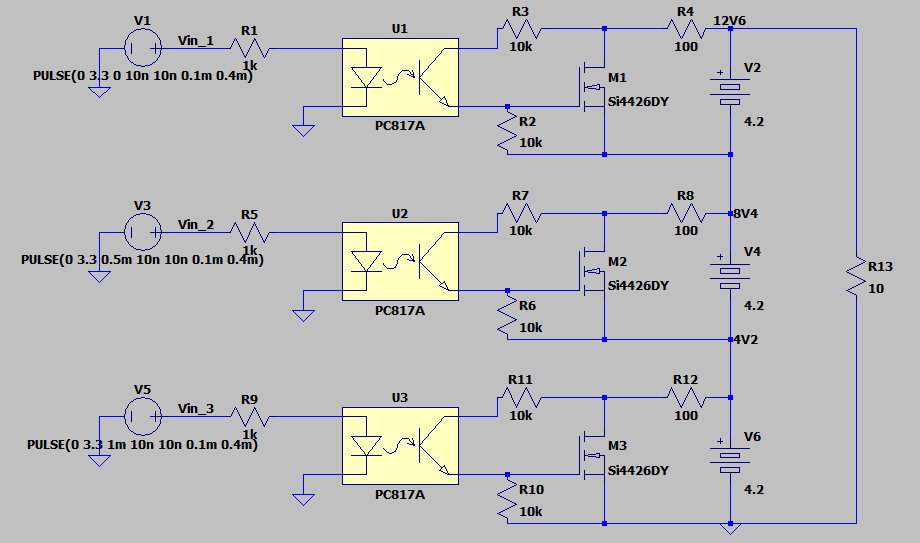
\includegraphics[scale=0.5]{./Figures/HW/simulation-balance.png}
    \caption{Simulating the Cell-Balancing Circuit on LTSpice}
    \label{fig:hw-balance-circuit}
\end{figure}

\begin{figure}[h!]
    \centering
    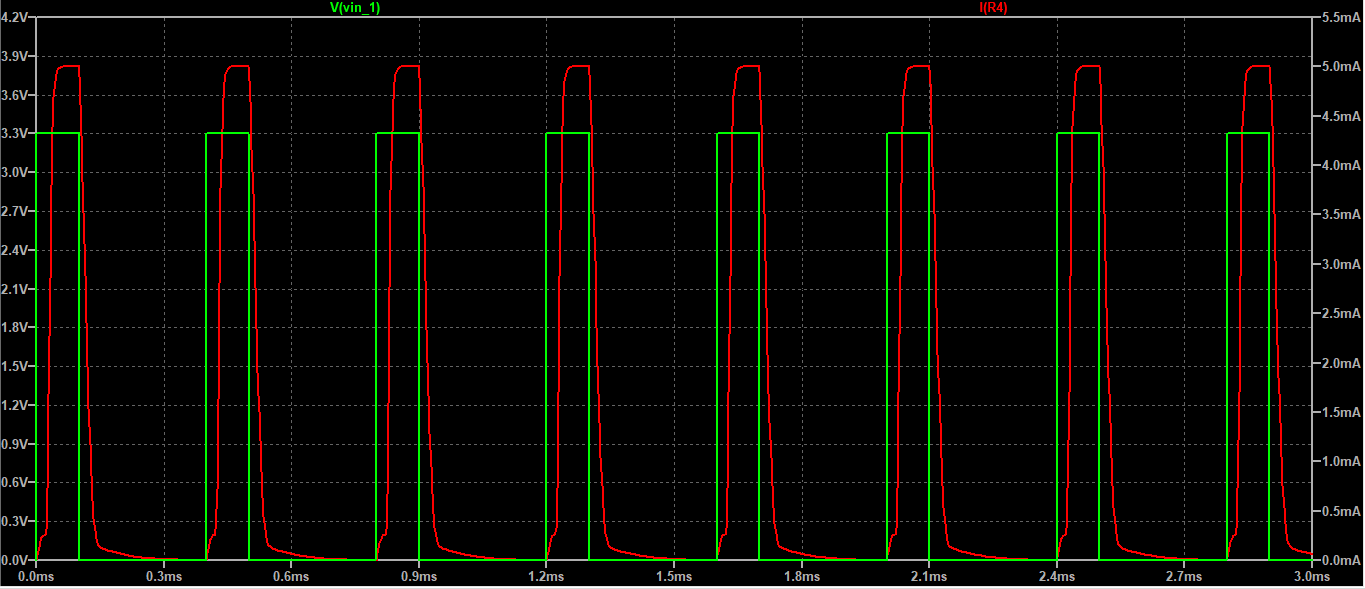
\includegraphics[scale=0.35]{./Figures/HW/results-balance.png}
    \caption{The results of simulation. $Vin_1$ in green, Current through $R_4$ in red.}
    \label{fig:hw-balance-results}
\end{figure}

\newpage

\subsection{Power Distribution}
After inserting a protection layer after the battery pack, its power is distributed all over the system. In order to provide stable connections from the power source to all system, a subsysystem of connectors, and power conversion is required.
In order to achieve proper connection, these connectors are used:
\begin{itemize}
	\item XT-60 Connector, which is a polarized connector for power input.
	\item Terminal and Barrier Terminal Blocks for power distribution.
	\item USB Type-A for to provide power to the SBC and other USB-powered peripherals if needed.
	\item Flat Terminals for fast debugging.
\end{itemize}

Although the input power connector is polarized, there is a possibility for reverse power connection, which would cause immediate damage to all peripherals. A simple solution for this problem is simple inverse polarity protection circuit. For a low power applications, a single diode can be enough. However, in the case of this robot, up to more than \textbf{3 W} of power can be wasted on the diode. A Schottky diode can result in a less power loss, but more efficiency is required.

\begin{figure}[h!]
	\centering
	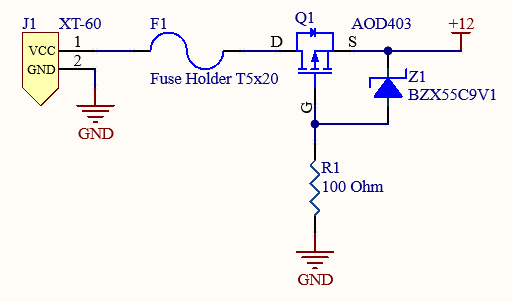
\includegraphics[scale=0.6]{./Figures/HW/reverse-polarity.png}
	\caption{Improved Reverse Polarity Protection}
	\label{fig:hw-reverse}
\end{figure}

An alternate solution is building a reverse-polarity protection circuit, based on a \textbf{P-Channel MOSFET} shown in figure \ref{fig:hw-reverse}, whose power loss depends mainly on its Drain-Source Resistance [$R_{DS(on)}$], which can be as low as $7 m\Omega$ at Gate-Source Voltage $[V_{GS}] = \textbf{-9 V}$ \cite{AOD403-datasheet}


To obtain a stable \textbf{5 V} source, a buck converter is used to obtain \textbf{5 V} from the battery pack. Another parameter to take in mind is choosing a suitable buck-converter, capable of supplying the demanded current without a compromise. Most current draw comes from the SBC and servo motors, up to about \textbf{5 A}. A suitable buck-converter module was the one based on \textbf{XL4016}, capable of producing up to 8A, as well as including many protection features, like: thermal shutdown, and short circuit protection \cite{XL4016-datasheet}.

\newpage

\begin{figure}[h!]
	\centering
	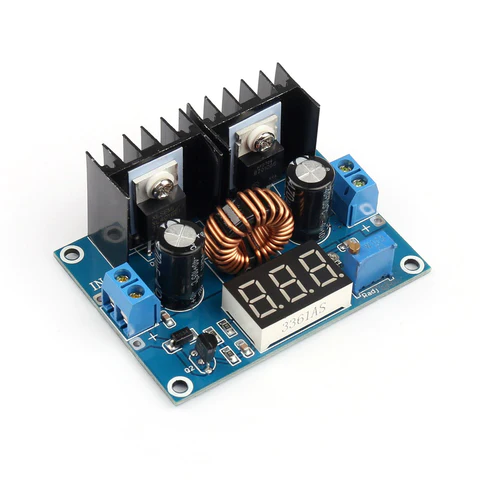
\includegraphics[scale=0.5]{./Figures/HW/xl4016.png}
	\caption{The used buck converter based on XL4016}
	\label{fig:hw-buck}
\end{figure}

One final measure of safety is fuses at both before and after conversion. From power calculations, fuses of rating \textbf{6 A} and \textbf{5 A} is added after the battery pack and the converter respectively.

\subsection{Auxiliary Boards}

A number of interfacing circuits have been designed to aid in the data gathering, motor and arm control via multiple microcontroller units. All the circuit were designed to support an STM32F103C8T6: the reason behind using it and how it is used will be discussed in detail next chapter. The designed circuits are as follows:
\begin{itemize}
	\item \textbf{Actuator Board:} Supports up to 10 servo motor inputs to microcontroller.
	\item \textbf{Motor Board:} Has inputs for 4 motors and 4 magnetic encoders to microcontroller.
	\item \textbf{Sensors Board:} Supports up to 4 Ultrasonic sensors and a 6 or 9 DOF IMU sensor.
	\item \textbf{VLC Receiver Prototype Board:} Able to read visible light signal for proximity localization via the onboard photodiode accompanied with aiding circuitry. The idea of operation of this VLC receiver will discussed in chapter~\ref{ch:loc}.
\end{itemize}

\newpage

\section{Output}

\subsection{Schematics}

\begin{figure}[h!]
	\centering
	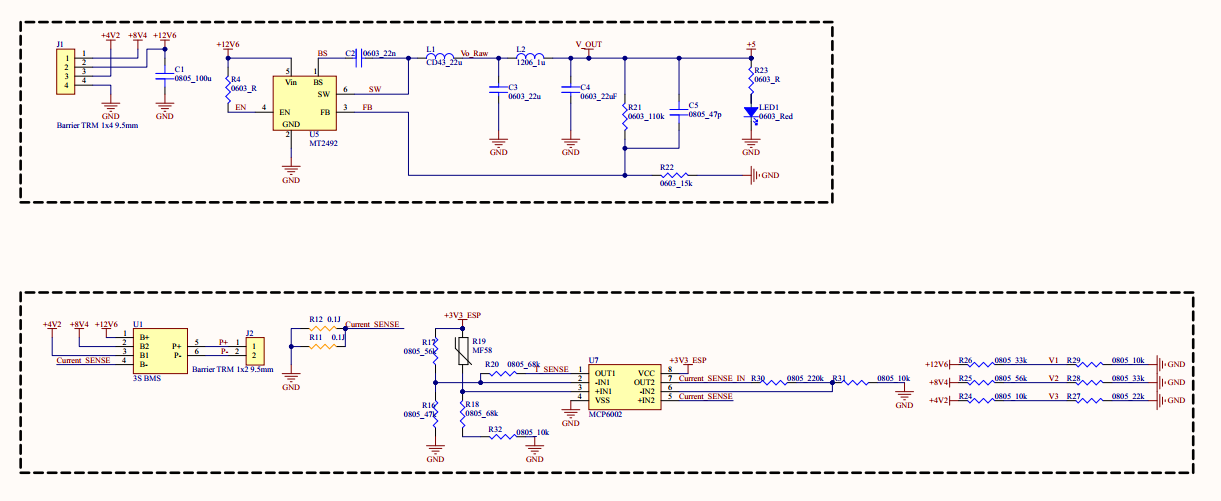
\includegraphics[scale=0.4]{Figures/HW/schem-bms-1.png}
	\caption{BMS Board Schematic -- Voltage Conversion for controller (Top) Measurement Modules and Protection Module (Bottom)}
	\label{fig:hw-bms-schem-1}
\end{figure}

\begin{figure}[h!]
	\centering
	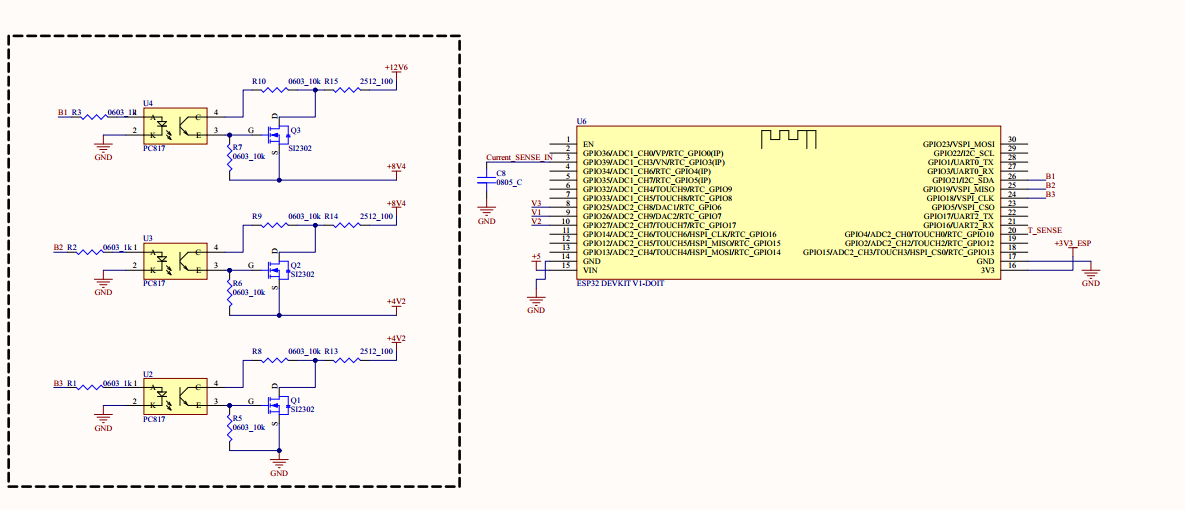
\includegraphics[scale=0.4]{Figures/HW/schem-bms-2.png}
	\caption{BMS Board Schematic -- Cell-Balancing circuit ESP32 Controller}
	\label{fig:hw-bms-schem-2}
\end{figure}

\begin{figure}[h!]
	\centering
	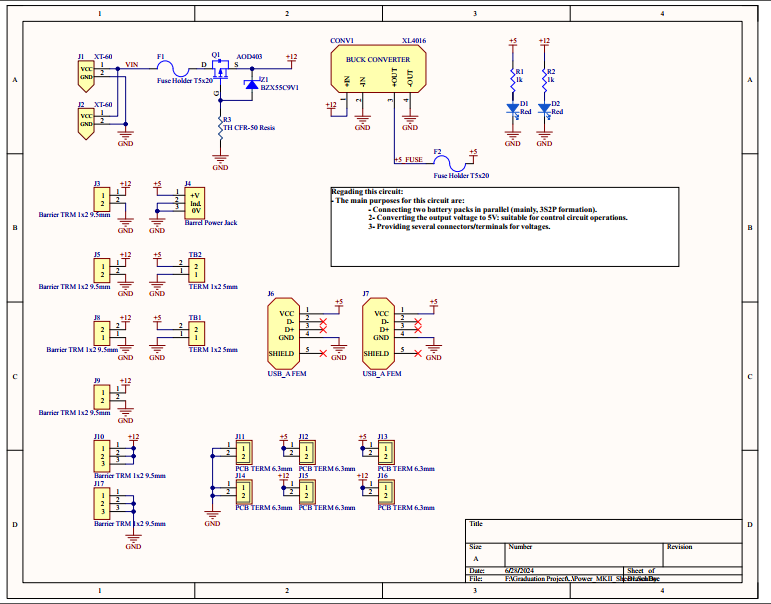
\includegraphics[scale=0.4]{Figures/HW/schem-pwr.png}
	\caption{Power Distribution Board Schematic}
	\label{fig:hw-pwr-schem}
\end{figure}

\newpage

\begin{figure}[h!]
	\centering
	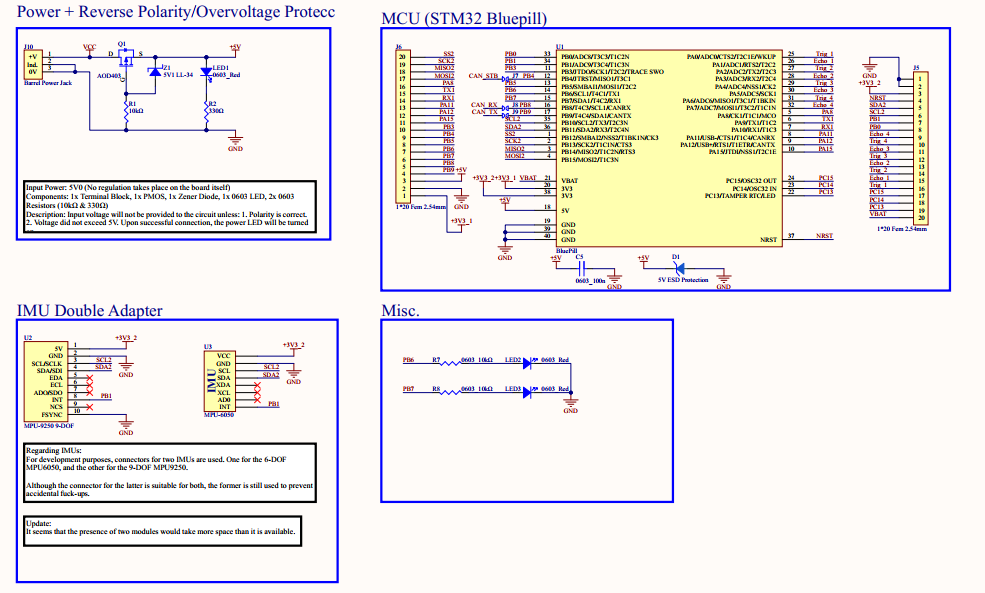
\includegraphics[scale=0.4]{Figures/HW/schem-sensi-1.png}
	\caption{Sensors Board Schematic -- First Part}
	\label{fig:hw-sensi-schem-1}
\end{figure}

\begin{figure}[h!]
	\centering
	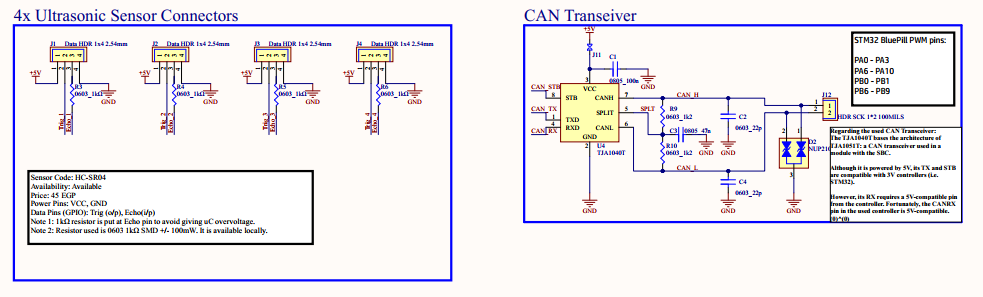
\includegraphics[scale=0.4]{Figures/HW/schem-sensi-2.png}
	\caption{Sensors Board Schematic -- Second Part}
	\label{fig:hw-sensi-schem-2}
\end{figure}

\begin{figure}[h!]
	\centering
	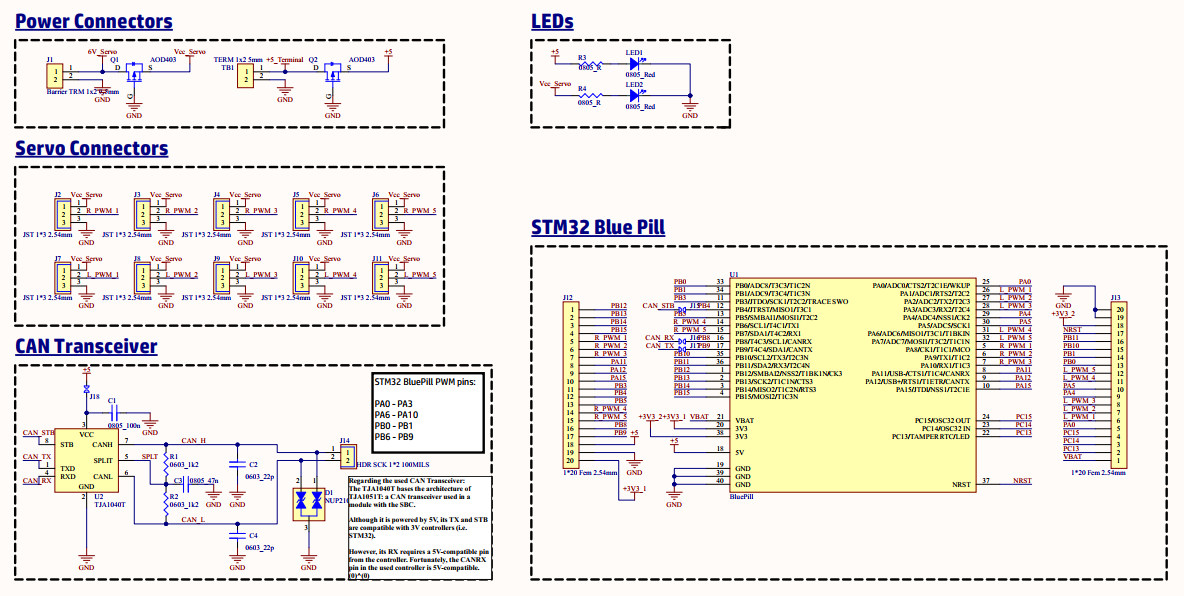
\includegraphics[scale=0.4]{Figures/HW/schem-actuators.png}
	\caption{Actuator Board Schematic}
	\label{fig:hw-servo-schem}
\end{figure}

\newpage

\begin{figure}[h!]
	\centering
	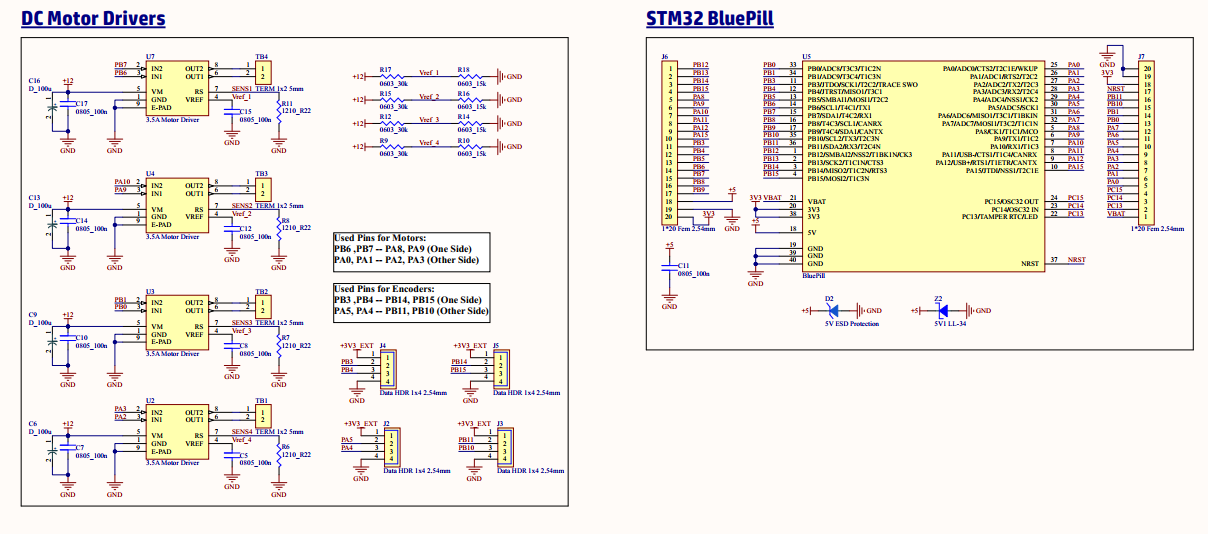
\includegraphics[scale=0.4]{Figures/HW/schem-motor-1.png}
	\caption{Motion Board Schematic -- First Part}
	\label{fig:hw-motion-schem-1}
\end{figure}

\begin{figure}[h!]
	\centering
	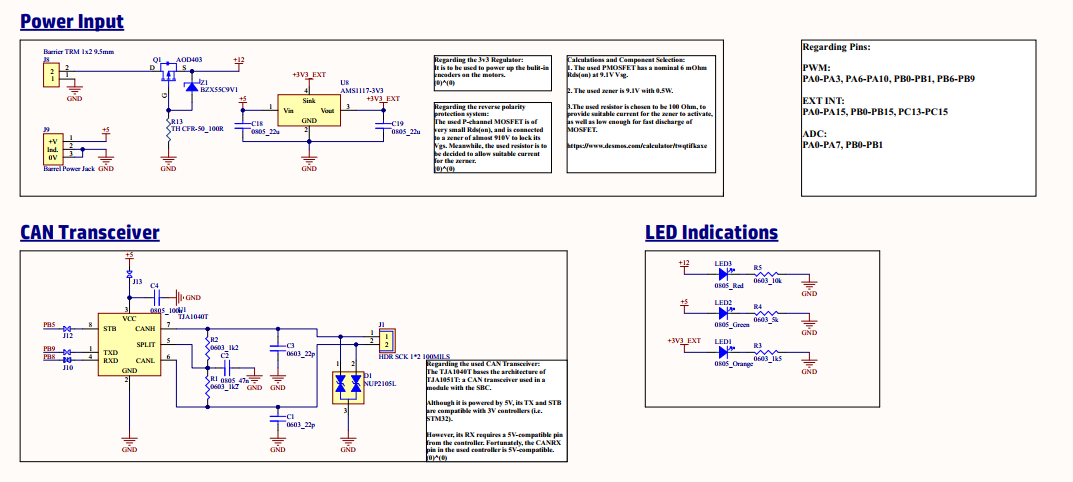
\includegraphics[scale=0.4]{Figures/HW/schem-motor-2.png}
	\caption{Motion Board Schematic -- Second Part}
	\label{fig:hw-motion-schem-2}
\end{figure}


\begin{figure}[h!]
	\centering
	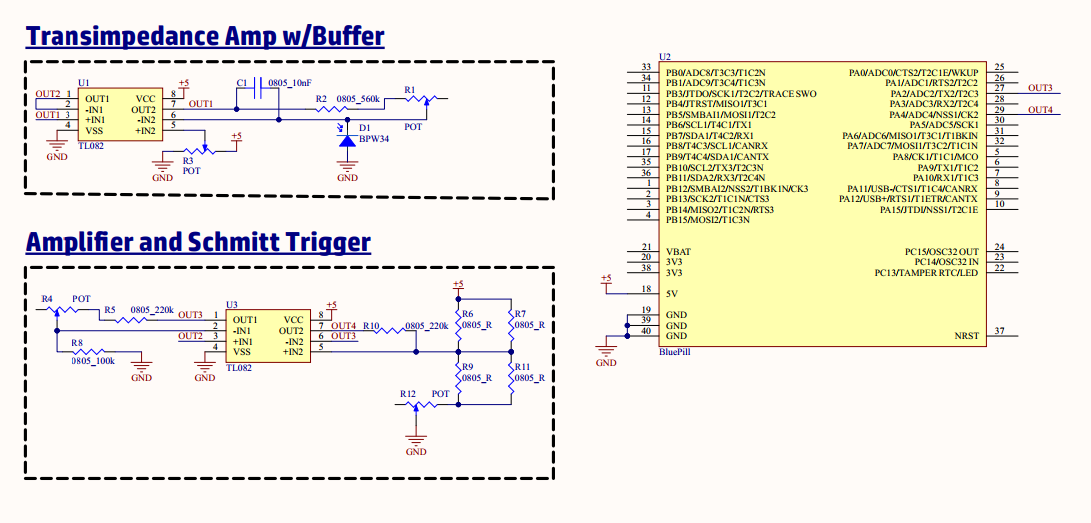
\includegraphics[scale=0.4]{Figures/HW/schem-vlc.png}
	\caption{VLC Receiver Board Schematic}
	\label{fig:hw-vlc-schem-}
\end{figure}


\newpage


\subsection{PCB Designs}

\vspace{3mm}

\begin{figure}[h!]
	\centering
	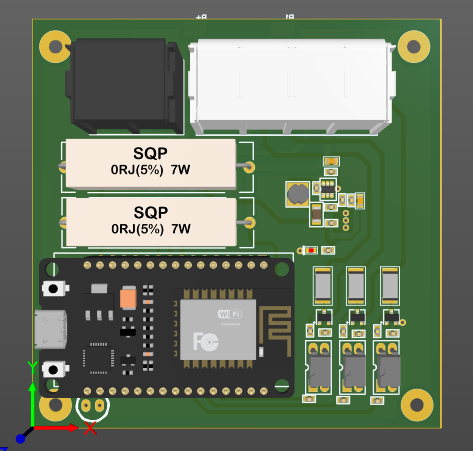
\includegraphics[scale=0.8]{Figures/HW/pcb-bms.png}
	\caption{BMS Board PCB}
	\label{fig:hw-bms-pcb}
\end{figure}



\begin{figure}[h!]
	\centering
	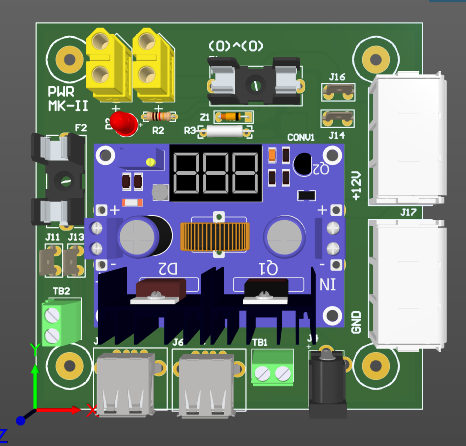
\includegraphics[scale=0.8]{Figures/HW/pcb-power.png}
	\caption{Power Distribution Board PCB}
	\label{fig:hw-pwr-pcb}
\end{figure}

\newpage

\begin{figure}[h!]
	\centering
	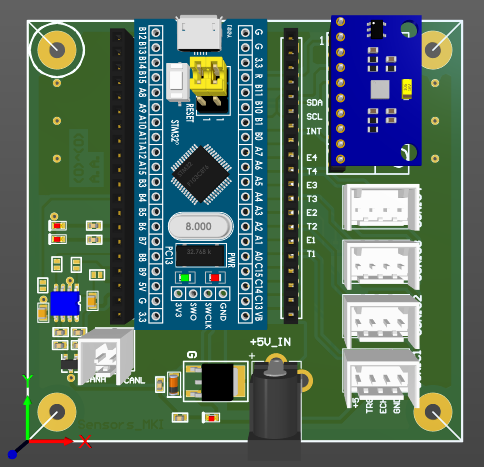
\includegraphics[scale=0.8]{Figures/HW/pcb-sensi-boi.png}
	\caption{Sensors Board PCB}
	\label{fig:hw-sense-pcb}
\end{figure}


\begin{figure}[h!]
	\centering
	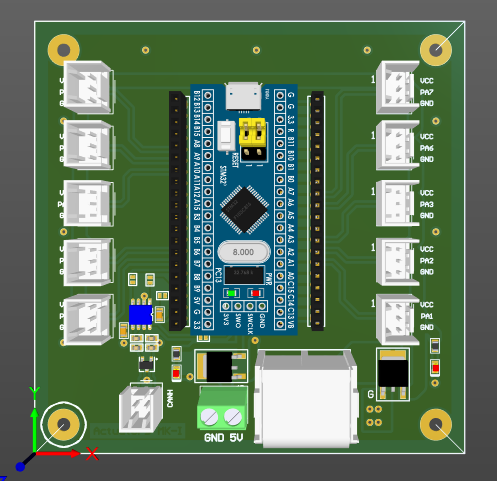
\includegraphics[scale=0.8]{Figures/HW/pcb-actuator.png}
	\caption{Actuator Board PCB}
	\label{fig:hw-servo-pcb}
\end{figure}

\newpage

\begin{figure}[h!]
	\centering
	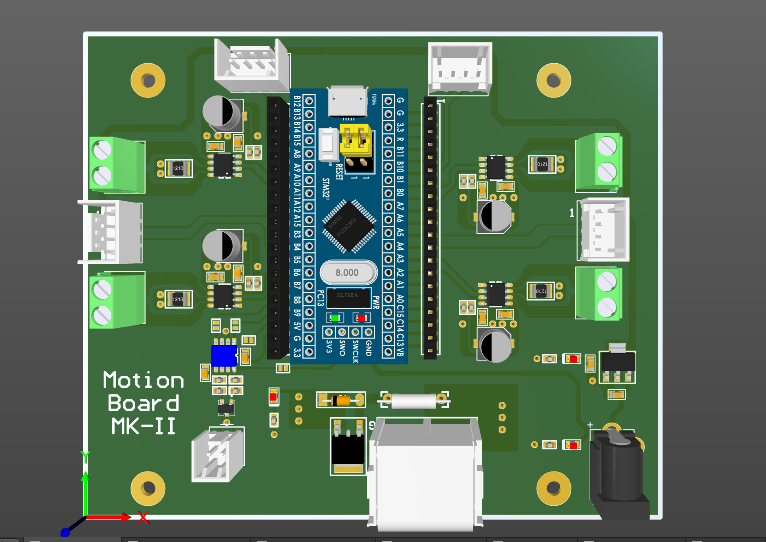
\includegraphics[scale=0.8]{Figures/HW/pcb-motor-mk-ii.png}
	\caption{Motion Board PCB}
	\label{fig:hw-motion-pcb}
\end{figure}



\begin{figure}[h!]
	\centering
	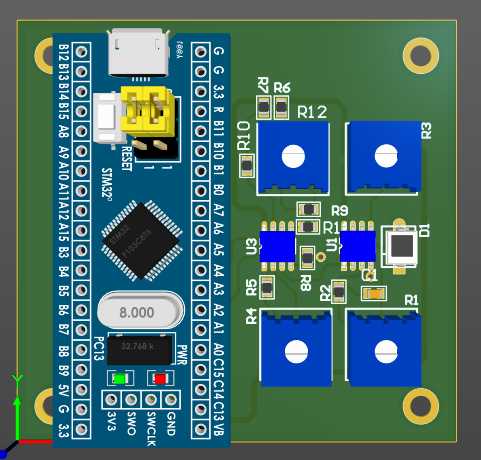
\includegraphics[scale=0.8]{Figures/HW/pcb-vlc.png}
	\caption{VLC Receiver Board PCB}
	\label{fig:hwvlc-pcb}
\end{figure}







% For current draw of about \textbf{4 A} (from subsection \ref{subsection:battery}), 
%Hello there
% I have already added that reference, so don't worry

%Honestly, I am too tired right now.
%I will finish this...I hope
%You know, it is not easy to do stuff you feel it does not fit you. You get a sense of "hey, I can do something even better for myself instead. It can be as lazy as laying down on bed doing nothing."

% you know, that reminds me of a story, you see there was a gro



%%%%%%%%%%%%%%%%%%%%%%%%%%%%%%%%%%%%%%%%%%%%%%%%%%%%%%%%%%%%%%%%%%%%%%%%%%%%%%%%%
\newpage
\chapter{Sensing \& Control}
\section{Introduction}
In this chapter, the proposed electrical and electronic infrastructure model will be thoroughly examined---purely from a sensors'/embedded systems' perspective; along with the development objectives in mind to achieve the desired performance.

% oi
%io
%Something on your mind ?
% nope... why?

%no reason really..I sometimes struggle  with words. Heck, even till this day.
%I am sure yor (you're XDD) more comptent though.
%I swear I was gonna fix this XD
% not really. you give me too much credit and yourself too little.
% you are WAAAY more capable than you think you are.
%I..well..am at lost of words, really.. UwU
%I will go back now
% alrighty, bro. Imma check on your work once I am finished with the dumpster fire I am working on

% I am praying for you
% <3

\section{Development Objectives}
A robot that is able to do all the objectives listed in chapter~\ref{ch:1} must need an incredible amount of data and precise control. Ergo, the robot must be equipped with a wide range of sensors that complements each other and provide the desired level of control. The list of following objectives will be framed specifically from a data gathering and fine control perspective:
\begin{enumerate}
    \item There must be a way for the robot to detects rotation angle or linear displacement. For this, an \textbf{encoder} will be used at each motor.
    \item As the robot is moving, it should be able to detect if there is an obstacle in its path. For that, there needs to be \textbf{ultrasonic} sensors at each of its sides.
    \item The robot should be able to determine its speed and orientation in space. Therefore, it must be equipped with an \textbf{IMU} sensor.
    \item The robot's path should be streamed in real-time for the operator. Hence, a \textbf{camera} is needed.
    \item Fine motor control is needed and can be implemented via a \textbf{software PID controller}.
\end{enumerate}
\newpage

\section{Used Components and Software Tools} % + state reason behind using them
\vspace{-2mm}
The microcontroller-of-choice is the STM32F103C8T6---figure \ref{fig:stm32}: a CORTEX-M3 ARM microcontroller equipped with an array of useful peripherals, is powerful enough to handle data gathering, and supports ROS \cite{stm32-site}.
% maybe put a photo of blue pill + reference STMicroelectronics' official website/documentation
\vspace{-1mm}
% 
\begin{figure}[h!]
    \centering
    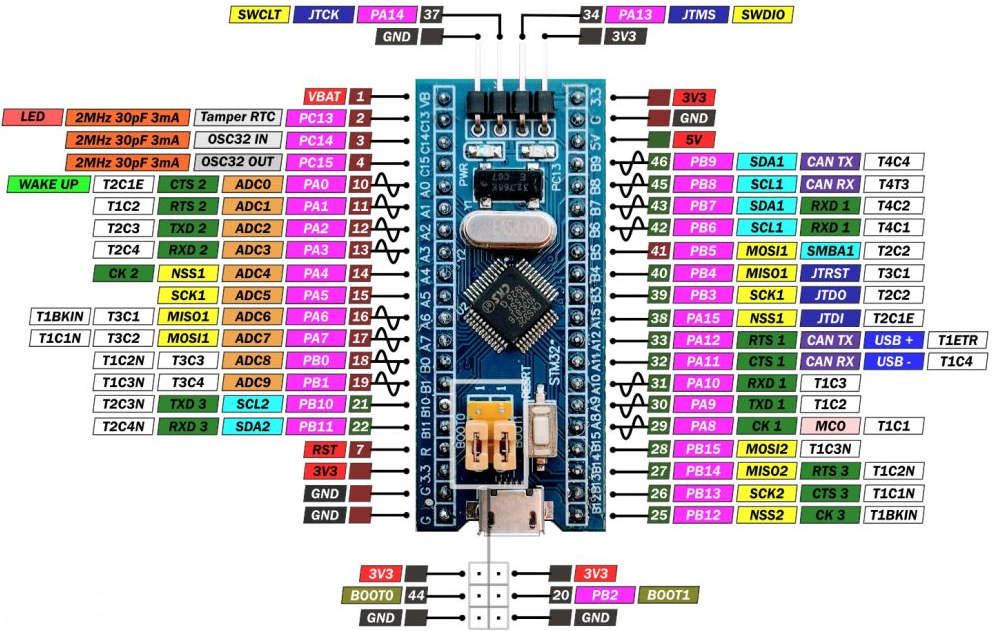
\includegraphics[scale=0.35]{./Figures/Ch4/stm32.png}
    \caption{Used Microcontroller}
    \label{fig:stm32}
\end{figure}

The used sensors are:
\vspace{-1mm}
\begin{enumerate}
    \item \textbf{Ultrasonic Sensors}
    \vspace{-1.5mm}
        \begin{itemize}
            \item Function: detect obstacles in the robot's path in a 1.5m radius.
            \vspace{-1mm}
            \item Used Peripheral: \textit{GPIO}.
            % photo
        \end{itemize}
    \item \textbf{MPU6050}
    \vspace{-1.5mm}
        \begin{itemize}
            \item Function: detect changes in motion via the included 3-axis gyroscope and 3-axis accelerometer. 
           \vspace{-1mm}
            \item Peripheral: \textit{I2C}.
            % photo
        \end{itemize}
    \item \textbf{Magnetic Encoders} 
    \vspace{-1.5mm}
        \begin{itemize}
            \item Function: an encoder is connected to each motor to detect and calculate rotation angle and linear displacements; primarily used to implement \textbf{PID control}.
            \vspace{-1mm}
            \item Used Peripheral: \textit{Timer}, \textit{Interrupts}, \textit{ADC}, \textit{PWM}.
            % photo
        \end{itemize}
\end{enumerate}

It was decided to use the Arduino platform for handling data gathering and control. There are multiple reasons for this:
\begin{enumerate}
    \item Open-source, widely-supported packages.
    \item Ease of integration with ROS.
\end{enumerate}

\newpage

\section{Design and Development Strategy}
In this section, the design and development principles used will be tackled. For additional information regarding any of the used sensors, go to appendix~\ref{ap:b}.
\subsection{Ultrasonic Implementation}
The principle of operation of ultrasonic sensors can be found in appendix~\ref{ap:b.us}. Based on that, the proposed design is composed mainly of the functions in code snippets \ref{cd:us1} to \ref{cd:us3}. The full code base can be found in the project's Github repository\footnote{Repository link: \url{https://shorturl.at/Ln4UO}}.
\vspace{3mm}
\lstinputlisting[language=C++, style=CodeStyleCpp, caption=Initialization Function For Ultrasonic Sensors, label=cd:us1, firstline=1, lastline=11]{./CodeSnippets/Sensors/Ultrasonic/ultrasonic.cpp}
% \lstinputlisting[language=C++, style=CodeStyleCpp, caption=Function to Detect Distance From Obstacle -- Front Sensor, label=cd:haha, firstline=12, lastline=24]{CodeSnippets/Sensors/Ultrasonic/ultrasonic.cpp}
% \lstinputlisting[language=C++, style=CodeStyleCpp, caption=Function to Detect Distance From Obstacle -- Back Sensor, label=cd:haha, firstline=25, lastline=37]{CodeSnippets/Sensors/Ultrasonic/ultrasonic.cpp}
\vspace{3mm}
\lstinputlisting[language=C++, style=CodeStyleCpp, caption=Function to Detect Distance From Obstacle -- Left Sensor, label=cd:us2, firstline=38, lastline=50]{./CodeSnippets/Sensors/Ultrasonic/ultrasonic.cpp}
\newpage
\lstinputlisting[language=C++, style=CodeStyleCpp, caption=Function to Detect Distance From Obstacle -- Right Sensor, label=cd:us3, firstline=51, lastline=63]{./CodeSnippets/Sensors/Ultrasonic/ultrasonic.cpp}
\vspace{-3mm}
\subsection{MPU6050 Implementation}
\vspace{-1mm}
The principle of operation of IMU's can be found in appendix~\ref{ap:b.imu}. For convenience, an arduino library is used to operate the sensor and extract the necessary data from it. Based on that, the proposed design is composed mainly of the code listed in code snippets \ref{cd:mpu1} to \ref{cd:mpu4}. The full code base can be found in the project's Github repository\footnote{Repository link: \url{https://shorturl.at/Ln4UO}}.

\vspace{1mm}
\lstinputlisting[language=C++, style=CodeStyleCpp, caption=Libraries Used For MPU6050, label=cd:mpu1, firstline=1, lastline=3]{./CodeSnippets/Sensors/MPU6050/mpu.cpp}
\lstinputlisting[language=C++, style=CodeStyleCpp, caption=Defined Variables For MPU6050, label=cd:mpu2, firstline=5, lastline=8]{./CodeSnippets/Sensors/MPU6050/mpu.cpp}
\lstinputlisting[language=C++, style=CodeStyleCpp, caption=Extracting Data From MPU6050 Buffer, label=cd:mpu4, firstline=24, lastline=29]{./CodeSnippets/Sensors/MPU6050/mpu.cpp}
\newpage
% \lstinputlisting[language=C++, style=CodeStyleCpp, caption=Initialization of I2C and MPU6050, label=cd:mpu3, firstline=10, lastline=22]{CodeSnippets/Sensors/MPU6050/mpu.cpp}


\subsection{Encoder Implementation}
\vspace{-1mm}
The principle of operation of encoders, as well as the idea behind PID can be found in appendix~\ref{ap:b.enc} and~\ref{ap:b.pid} respectively. The proposed design is composed mainly of the code listed in code snippets \ref{cd:enc1} to \ref{cd:enc6}. Additionally, the code implementation for PID is in code snippets \ref{cd:pid1} to \ref{cd:pid2}. The full code base can be found in the project's Github repository\footnote{Repository link: \url{https://shorturl.at/O9fj9}}.
\vspace{1mm}
\lstinputlisting[language=C++, style=CodeStyleCpp, caption=Defined Class For Encoder Interfacing, label=cd:enc1, firstline=1, lastline=13]{./CodeSnippets/Sensors/Encoder/encoder.cpp}


\lstinputlisting[language=C++, style=CodeStyleCpp, caption=Encoder Class Function For Speed Calculation, label=cd:enc2, firstline=15, lastline=25]{./CodeSnippets/Sensors/Encoder/encoder.cpp}

\newpage

\lstinputlisting[language=C++, style=CodeStyleCpp, caption=Encoder ISR Class, label=cd:enc3, firstline=27, lastline=39]{./CodeSnippets/Sensors/Encoder/encoder.cpp}

\lstinputlisting[language=C++, style=CodeStyleCpp, caption=Encoder ISR Functions, label=cd:enc4, firstline=47, lastline=60]{./CodeSnippets/Sensors/Encoder/encoder.cpp}

% \lstinputlisting[language=C++, style=CodeStyleCpp, caption=ISR Setup, label=cd:enc6, firstline=76, lastline=87]{CodeSnippets/Sensors/Encoder/encoder.cpp}
\lstinputlisting[language=C++, style=CodeStyleCpp, caption=Speed Control Function (1), label=cd:enc5, firstline=93, lastline=102]{./CodeSnippets/Sensors/Encoder/encoder.cpp}
\newpage
\lstinputlisting[language=C++, style=CodeStyleCpp, caption=Speed Control Function (2), label=cd:enc6, firstline=104, lastline=112]{./CodeSnippets/Sensors/Encoder/encoder.cpp}
\vspace{-3mm}
% \lstinputlisting[language=C++, style=CodeStyleCpp, caption=Speed Control Function (2), label=cd:enc7, firstline=114, lastline=145]{CodeSnippets/Sensors/Encoder/encoder.cpp}
% \lstinputlisting[language=C++, style=CodeStyleCpp, caption=Defined Variables For Encoder, label=cd:enc9, firstline=123, lastline=144]{CodeSnippets/Sensors/Encoder/encoder.cpp}

\lstinputlisting[language=C++, style=CodeStyleCpp, caption=Defined Class For PID, label=cd:pid1, firstline=1, lastline=14]{./CodeSnippets/Sensors/PID/pid.cpp}
\lstinputlisting[language=C++, style=CodeStyleCpp, caption=PID Class Function For Output Calculation, label=cd:pid2, firstline=17, lastline=30]{./CodeSnippets/Sensors/PID/pid.cpp}

\newpage

\subsection{Publishing Data}
The main principle of publishing data is using ROS messages that are transmitted using USB serial protocols, Additionally the following snippets from 4.15 to 4.18 showcases a simple publisher on the micro-controller. 
\vspace{1mm}
\lstinputlisting[language=C++, style=CodeStyleCpp, caption=Publisher declaration, label=cd:pub1, firstline=18, lastline=20]{./CodeSnippets/Sensors/Ultrasonic/Sensors.ino}
\vspace{1mm}
\lstinputlisting[language=C++, style=CodeStyleCpp, caption=Publisher initialization, label=cd:pub2, firstline=58, lastline=61]{./CodeSnippets/Sensors/Ultrasonic/Sensors.ino}
\vspace{1mm}
\lstinputlisting[language=C++, style=CodeStyleCpp, caption=Callback function, label=cd:pub3, firstline=66, lastline=66]{./CodeSnippets/Sensors/Ultrasonic/Sensors.ino}
\vspace{1mm}
\lstinputlisting[language=C++, style=CodeStyleCpp, caption=Publishing continuously, label=cd:pub4, firstline=81, lastline=83]{./CodeSnippets/Sensors/Ultrasonic/Sensors.ino}
Further details about ROS architecture and how it operates will be discussed in the next chapter.

%are you here ? :0
%remember that paper I used for temperature sensing? in what category should be cited ?
% what do you mean in which category? 
% I think @article or @inproceedings suits it 
\newpage
\section{Output}

\begin{figure}[h!]
     \centering
     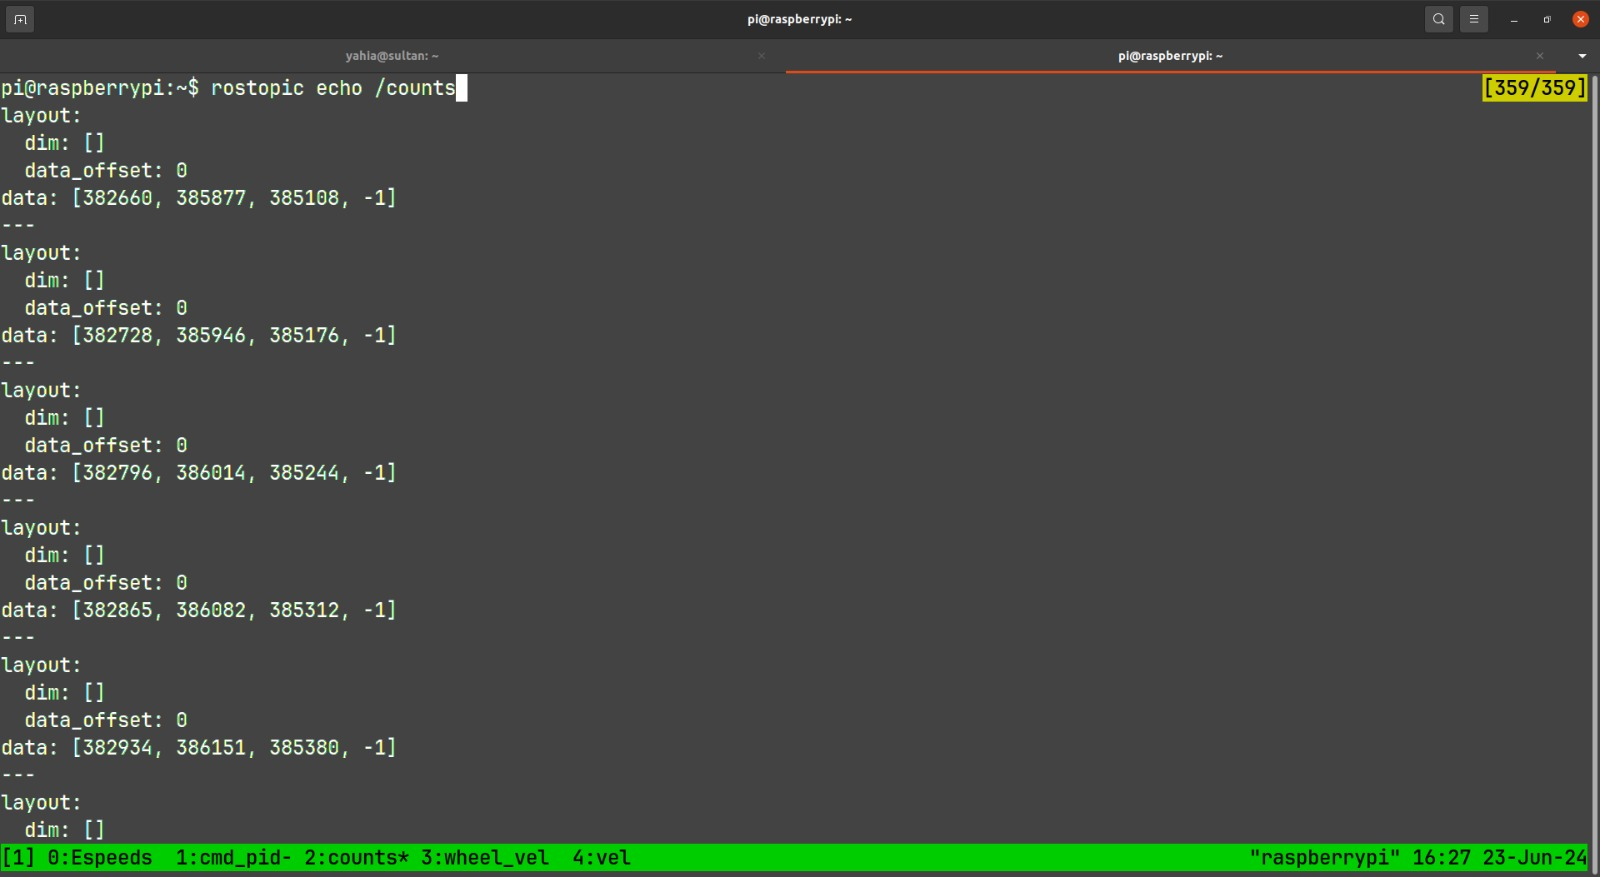
\includegraphics[scale=0.25]{./Figures/encoder.jpg}
     \caption{Encoders' Readings Sent Via ROSSerial and Displayed in Terminal}
     \label{fig:ref1}
\end{figure}

\begin{figure}[h!]
	\centering
	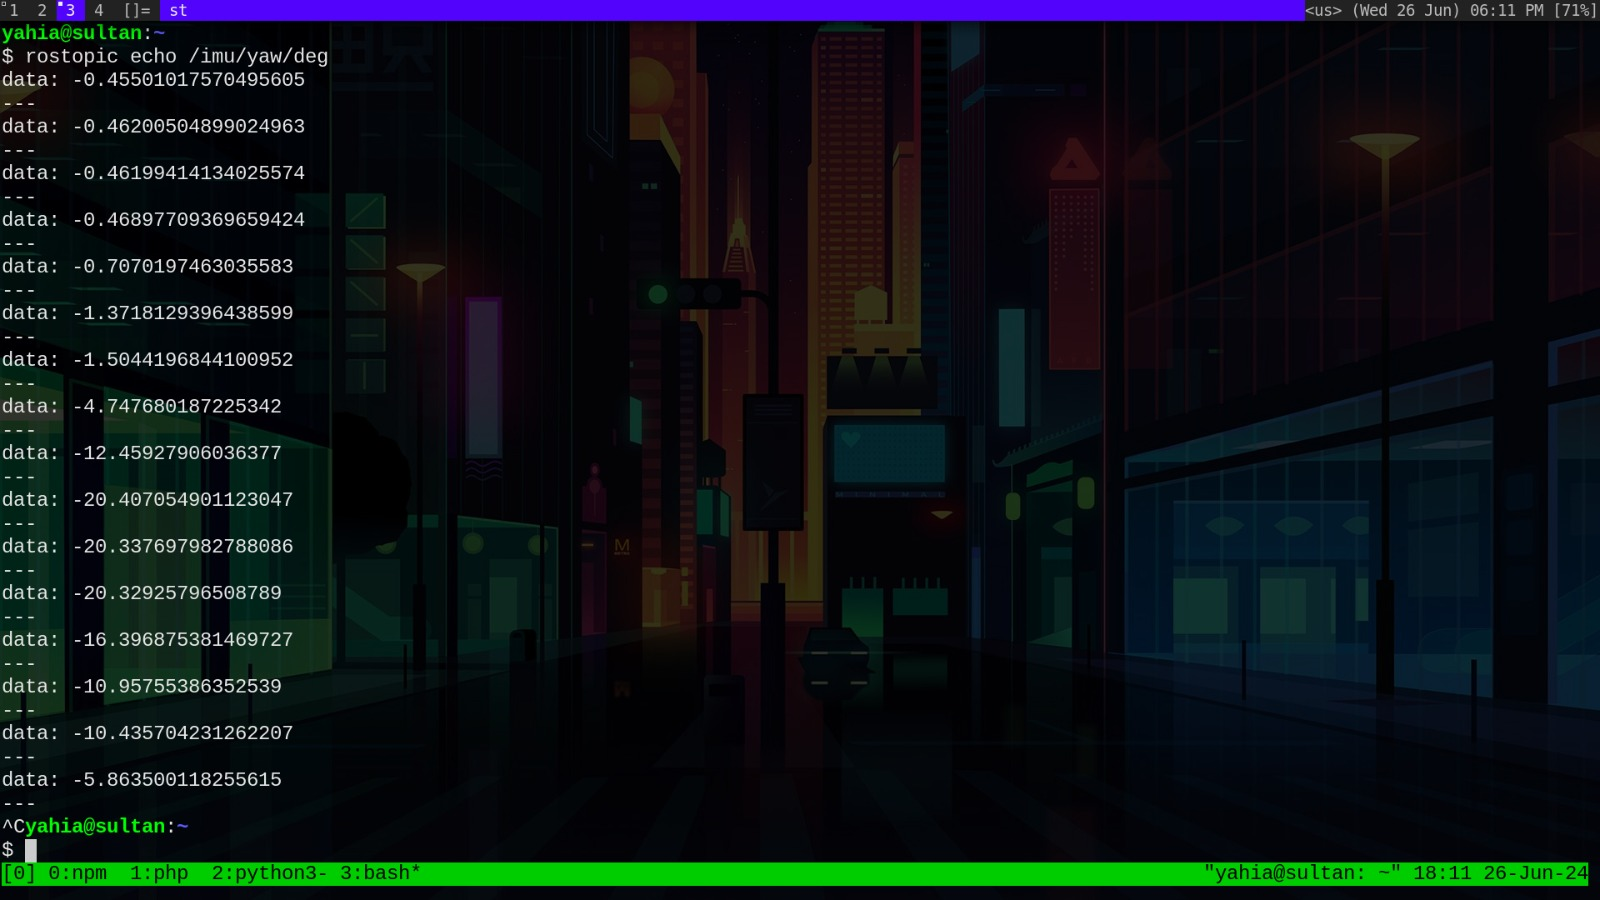
\includegraphics[scale=0.25]{./Figures/imu.jpg}
	\caption{IMU' Readings Sent Via ROSSerial and Displayed in Terminal}
	\label{fig:ref2}
\end{figure}






% \begin{figure}[h!]
%     \centering
%     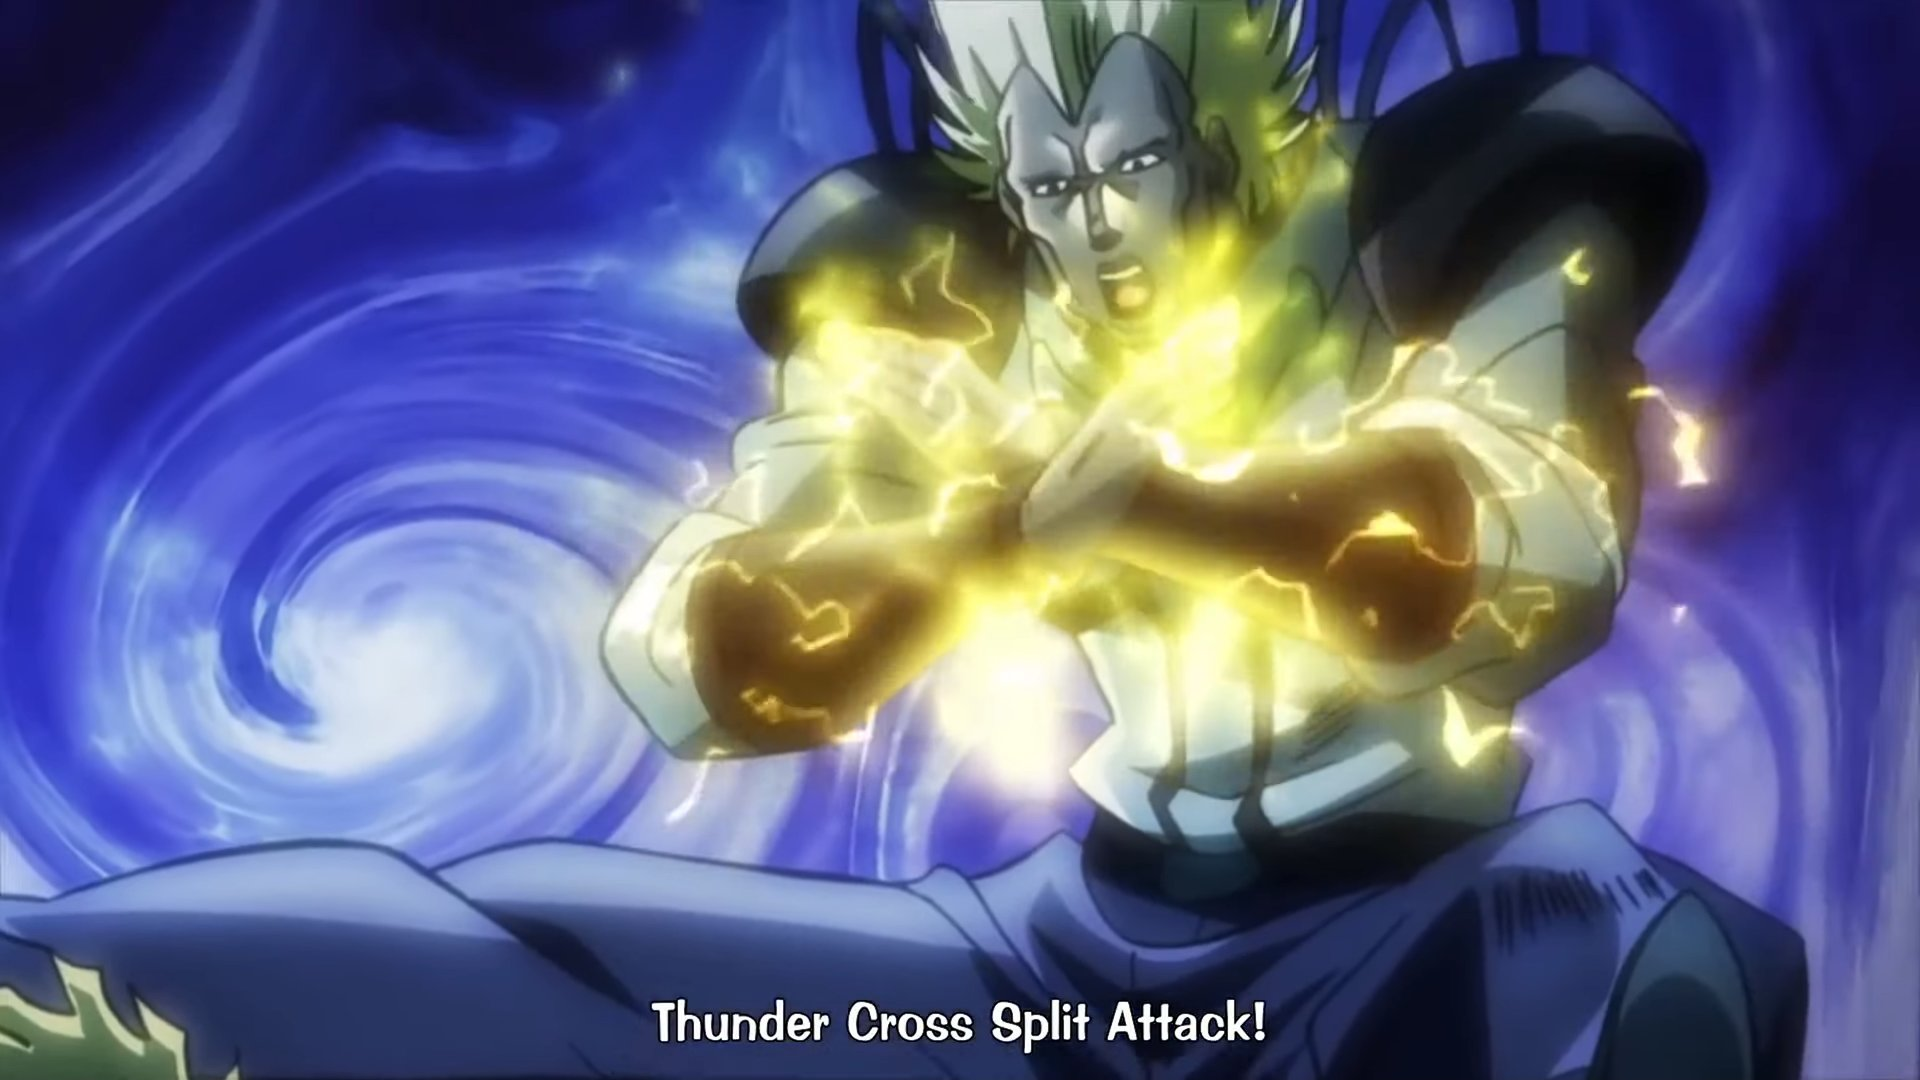
\includegraphics[scale=0.1]{Figures/fool.jpg}
%     \caption{You fell into my trap!}
%     \label{fig:ref1}
% \end{figure}
% \notrickroll

% \lstinputlisting[language=C, style=CodeStyleC, caption=test code, label=cd:haha, firstline=1, lastline=6]{CodeSnippets/haha.c}